%!TeX root = main.tex
\documentclass[main.tex]{subfiles}

\begin{document}

\chapter{Molecular simulation of adsorption}\label{adsorption}
\clearpage

Adsorption is the physical phenomenon by which a molecule, the adsorbate, attaches to a surface, the adsorbent. One particular application of adsorption in the industry is for gas separation, by using an adsorbent that specifically binds one constituent of the target gas mixture more than the other.

In this chapter, we detail the nature of this phenomenon in the case of small gases in zeolites. We then explain the usual techniques which are used for its numerical simulation, as well as a possible alternative.

\section{Molecular description}

\subsection{Physisorption and chemisorption}

The atomic nature of adsorption depends on the kind of chemical interaction that supports it. On the one hand, if the adsorbate forms a strong (\textit{i.e.} covalent, sometimes ionic) bond with the adsorbent, then the adsorption is called a chemisorption, because it involves a chemical reaction. In that case, the surface is modified. On the other hand, if the adsorbate and adsorbent are only bond by a weak interaction, the adsorption is called a physisorption and the surface is left intact.

Chemisorption involves a stronger bond that physisorption, and is thus less reversible. Since it changes the surface of the adsorbent, it cannot be used industrially to separate large amounts of gas, as the adsorbent would need to be provided in equivalently large amount. It can still be used as an intermediate step of a catalytic cycle that ends up regenerating the surface. In our case however, we will implicitly refer to physisorption when mentioning adsorption.

\subsection{Adsorption sites in crystalline materials}

\label{adsorptionsites}

%At the atomic scale, the movement of species is driven by quantum mechanics. While the exact formulation of Schr\"odinger's equation cannot be solved exactly for more than a few particles, it has long been approximated to give a global understanding of the relevant phenomenons. In this context, the forces that play a key role in the non-bonded interactions of species are usually divided into two components: the charges of the species, which contribute a Coulomb term that evolves in $\frac1r$ with the distance between two particles, and a Van der Waals term that decays to zero much faster.

An adsorption site designates a particular space where the adsorbate is likely to remain trapped on the surface of the adsorbent. In other words, the interaction between the adsorbate and the adsorbent is maximally attractive when the adsorbate is located in one of the adsorption sites.

The position of the adsorption site depends on the adsorbent, but also the adsorbate. At very low density for example, a small polar molecule like \ce{H_2O} will preferentially adsorb in locations where it can orient itself to maximize the stabilizing Coulomb interaction of the framework. A large apolar molecule like a xylene on the other hand, will adsorb in locations that maximize its Van der Waals interactions with the adsorbent. Such sites are not necessarily related.

Moreover, the location of the adsorption sites becomes less relevant when the density of the adsorbate becomes high. Indeed, the adsorbate-adsorbate interactions can play a key role in the global adsorption capacity of a material, and the stronger these interactions, the more the internal structure of the adsorbate will reorganize to accommodate these interactions, which may displace some molecules from the ideal adsorption site.

In the case of crystalline materials, adsorption sites can be identified through XRD spectroscopy. For example, \textcite{CO2SitesInMFI} identify the preferred adsorption sites for \ce{CO_2} in silica MFI zeolite (silicalite) in a context of very high mechanical pressure, compatible with DFT computations. Yet, the obtained positions for \ce{CO_2} molecules is not guaranteed to carry to another gas pressure than the one used in the study.

Overall, the situation is quite different from the cationic sites, discussed in \cref{sitehopping}, mostly because the cations cannot reach a ``high-density'' regime, given that their number is constrained by the number of aluminium atoms. In turn, this makes the use of site hopping or other site-derived algorithms less relevant in the context of adsorption simulation, except in the low-pressure regime.

\subsection{Small gases in zeolites}

Small gases such as \ce{CO_2}, \ce{N_2}, \ce{O_2}, \ce{CH_4} or \ce{Ar}, among others, are typical adsorbates that need to be separated for industrial purposes, be it for carbon capture, medical \ce{O_2} packaging, cold generation with \ce{N_2} or \ce{He}, and many other applications. In general, molecular sieves like zeolites can be used for this purpose

To separate molecules with significant size disparities, a simple approach consists in using a framework whose pore size allows one of the molecule to enter and adsorb, but not the other. Given the proximate sizes of the previous species however, this method cannot be used to separate these gases. Instead, what plays a key role is the adsorption capacity of the material with respect to each of these gases: if there is a material that adsorbs \ce{CO_2} easily but not \ce{N_2} for instance, then it can be used to separate the two.

\begin{figure}
	\centering
	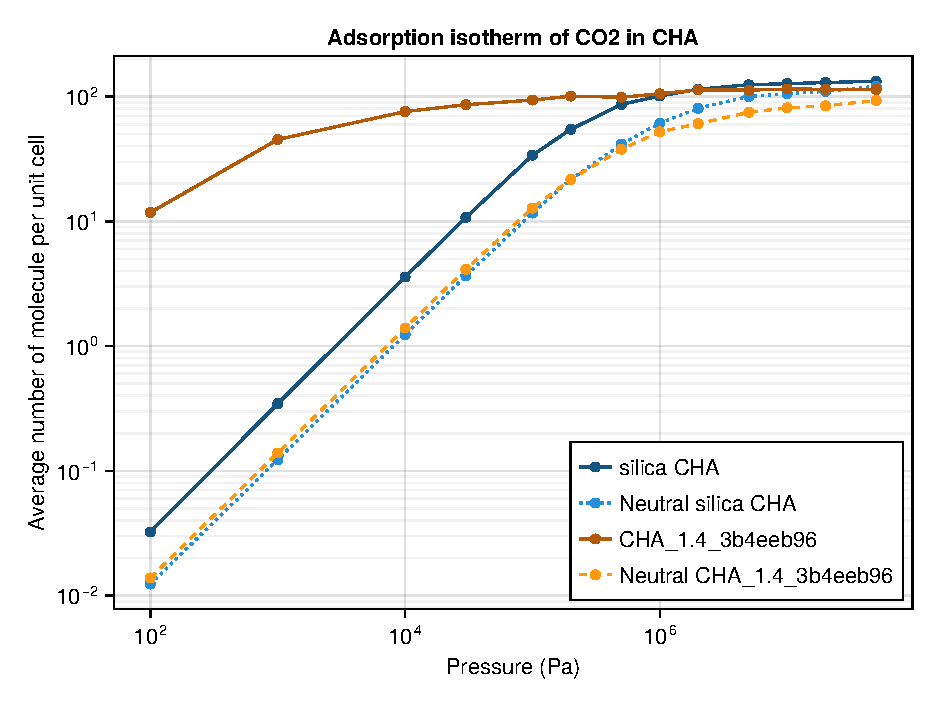
\includegraphics[width=\linewidth]{figures/gcmc/CO2CHANeutral.pdf}

	\caption{Adsorption isotherms of \ce{CO_2} on CHA at $\SiAl = \infty$ or \num{1.4}, with and without charges}\label{fig:CO2CHANeutral}
\end{figure}

In that regard, both van der Waals and Coulomb components of the framework-guest interaction energy need to be taken into account, as \cref{fig:CO2CHANeutral} illustrates in the case of \ce{CO_2} adsorption in zeolite CHA. The adsorption isotherms (see \cref{isotherms} for the definition) were computed for \ce{CO_2} in CHA with two \SiAl ratios: $\infty$ (\textit{i.e.} fully silicic) and \num{1.4}, using a fixed placement of both aluminiums and cations. In both cases, one isotherm was computed using the full force field from \textcite{BoulfelfelSholl2021}, while on the other, all the atoms of the framework (and the cations) were set to be neutral.

In the silicic case, the loading is \num{2.8\pm0.2} times higher with than without charges for the low/medium pressures (lower than \qty{0.5}{MPa}), then the difference starts to decrease. Therefore, while the porous volume, which roughly defines the van der Waals interaction, is the most important parameter for the global adsorption capacity in that case, the electrostatic interactions also plays a critical role.

That role becomes considerably more important for the cationic zeolite however, where the difference of loading with and without charges is of multiple orders of magnitude, and the absolute loading is much higher than in the silicic case for the low/medium pressures. At high pressure, the pores are already filled with gas so the trend becomes different: since the cation occupy some space, they leave less room for \ce{CO_2}, which explains why the loading becomes higher in the silicic zeolite.

Hence, the electrostatic interactions are the main adsorption drive in cationic zeolites are low/medium pressures. Otherwise, \textit{i.e.} for silicic zeolites or at high pressure, the van der Waals interactions are the most important parameter, although the coulombic interactions continue to play a key role.


\section{Grand Canonical Monte Carlo}
\label{GCMC}

\subsection{Principle}

The adsorption capacity of a gas in a material at a fixed temperature and pressure is the number of molecules of gas that are retained by the material when in contact with a gas in these conditions, at equilibrium. Since it is a macroscopic observable $\mathcal O$, which can be experimentally measured, it can also be expressed as the statistical average of its microscopic counterpart $o$ in a well-chosen statistical ensemble. For the current case, the adsorption capacity results from a chemical equilibrium between the gas out of the material, at its given temperature $T$ and pressure $P$, and the gas in the pores of the material, at the same temperature $T$. The pressure of the gas in the material is an ill-defined concept, because it depends on the density of the gas, which itself is not uniform at any mesoscopic scale in a porous material. Instead, the chemical equilibrium translates to the equality of the chemical potentials $\mu$ of the gas in both conditions, hence $\mu$ is the relevant statistical variable to describe the system in the material, which accounts for the fixed gas pressure $P$ out of the material. Finally, we will focus on rigid crystalline materials, hence the volume $V$ of a unit cell can be used as an extensive variable to limit the size of the system.

The statistical ensemble resulting from the constraints of fixing the chemical potential $\mu$, the temperature $T$, and the volume $V$ is called the grand canonical ensemble. Similar to \cref{eq:canonicalensemble} used for the canonical ensemble (where the number of particles $N$ is fixed instead of their chemical potential $\mu$), $\mathcal O$ can be expressed using an integral over the microstates $(N,\boldsymbol p_N)$:
\[\mathcal O = \left<o\right> = \frac1\Xi\sum_N\int\!\text d{\boldsymbol p_N}\  o\left({\boldsymbol p_N}\right)\exp\left(-\beta U\left({\boldsymbol p}\right) + \mu N\right)\label{eq:grandcanonicalensemble}\]
where $\beta = 1/k_BT$, $N$ is the number of gas particles, $\boldsymbol p_N$ is their configuration, and $\Xi$ is the grand canonical partition function.

Likewise, this integral can be numerically evaluated by relying on a Monte Carlo Markov Chain to provide a sequence of configurations $(N, \boldsymbol p_N)$ such that the statistical average $\left<o\right>$ can be retrieved by computing the arithmetic average of $o\left({\boldsymbol p_N}\right)$ over these configurations: this particular kind of simulation is naturally called a grand canonical Monte Carlo (GCMC) simulation. In the specific case of the adsorption capacity, the microscopic function is simply $o\left({\boldsymbol p_N}\right) = N$, thus it is computed by running a GCMC simulation and simply averaging the number of particles in the system across the simulation.

\subsection{Implementation}
\label{gcmc_implementation}

In practice, GCMC is implemented like a canonical MC simulation with one additional element: a swap MC move that can either insert or delete a particle. The insertion move simply consists in adding one additional gas particle to the system, while the deletion move removes one. If there are no particle in the systems anymore, the deletion move systematically fails; yet, it is crucial that the probability of trying an insertion or a deletion remains equal independently of the number of particles in the system, to ensure micro-reversibility. For this reason, only the probability of trying a swap move is specified as a simulation parameter, while the probability of trying either an insertion or a deletion cannot be individually chosen and are necessarily equal to half the probability of a swap move.

The acceptance probability of a swap move is not decided purely on the basis of the difference of energy in the system, as is the case in \cref{eq:MCcanonicalaccept} for the canonical ensemble, because it also depends on the chemical potential $\mu$ of the system. With $N$, the number of particles in the system before the trial swap move, and $\Delta E$ the energy difference between before and after the move, the acceptance probabilities for insertion and deletion are:
\[\begin{split}
	P_\text{accept}(\Delta E, N\to N+1) &= \min\paren{1,\ \frac{\beta\varphi P V}{N+1}\exp\paren{-\beta\Delta E}}\\
	P_\text{accept}(\Delta E, N\to N-1) &= \min\paren{1,\ \frac{N}{\beta\varphi P V}\exp\paren{-\beta\Delta E}}
\end{split}\]
The dependency to the chemical potential $\mu$ is conveyed by the pressure $P$ of the gas exterior to the zeolite. This value is corrected by the fugacity coefficient $\varphi$, which accounts for the difference between the real gas and the ideal gas model.

While the pressure $P$ and volume $V$ of the systems are simulation inputs, the fugacity coefficient $\varphi$ of the gas needs to be computed prior to the simulation. To do so, RASPA uses the Peng-Robinson equation of state \autocite{PengRobinson}, which is adequate for many common fluids. Since the range of gas applications I study is more restricted than the general-purpose RASPA software, I decided to use the GERG-2008 \autocite{GERG2008} equation of state, which is the ISO standard for natural gases due to its accuracy compared to experimental measurements, with an extended validity range up to \qty{700}K and \qty{70}{MPa}, in the scope of this study.

\begin{figure}
	\centering
	\begin{subfigure}{0.5\columnwidth}
		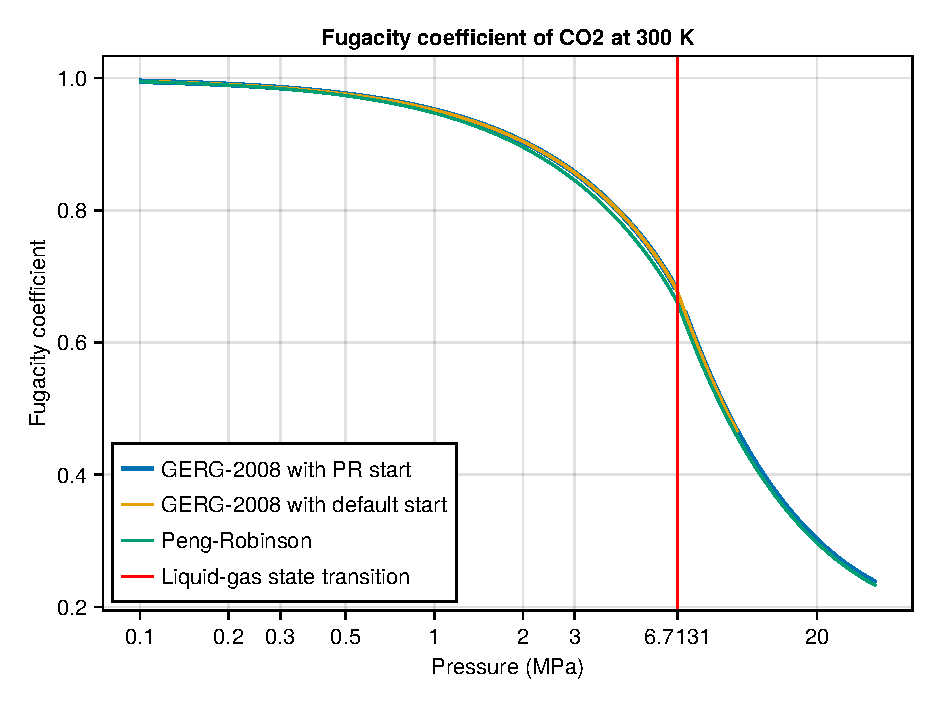
\includegraphics[width=\columnwidth]{figures/gcmc/fugacity.pdf}
		\subcaption{\ce{CO_2} at \qty{300}K}\label{fugacityCO2}
	\end{subfigure}\hfill%
	\begin{subfigure}{0.5\columnwidth}
		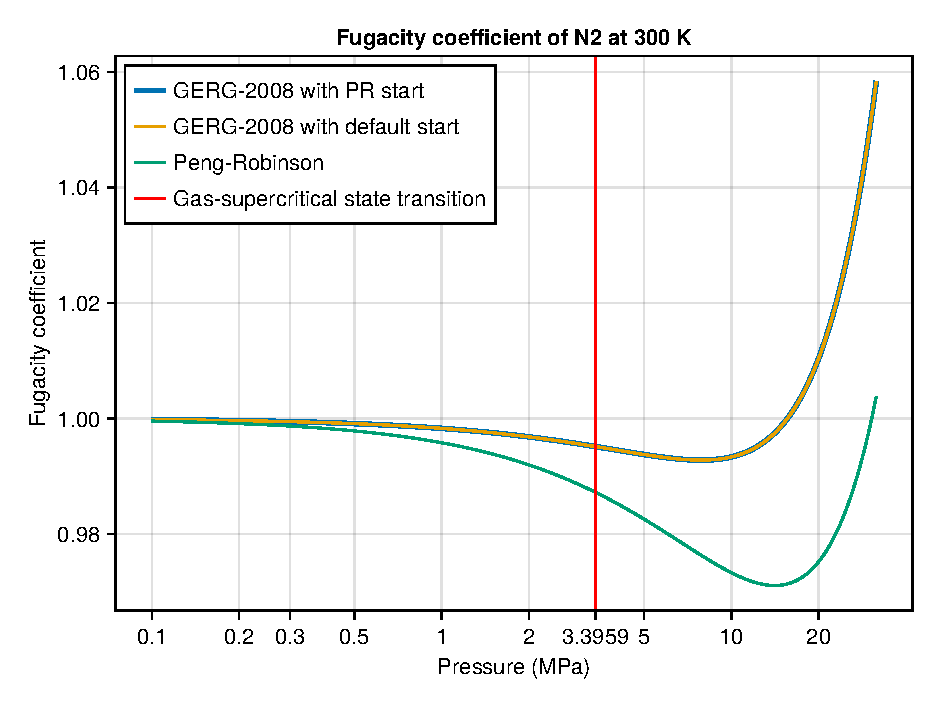
\includegraphics[width=\columnwidth]{figures/gcmc/fugacity_N2.pdf}
		\subcaption{\ce{N_2} at \qty{300}K}
	\end{subfigure}

	\begin{subfigure}{0.5\columnwidth}
		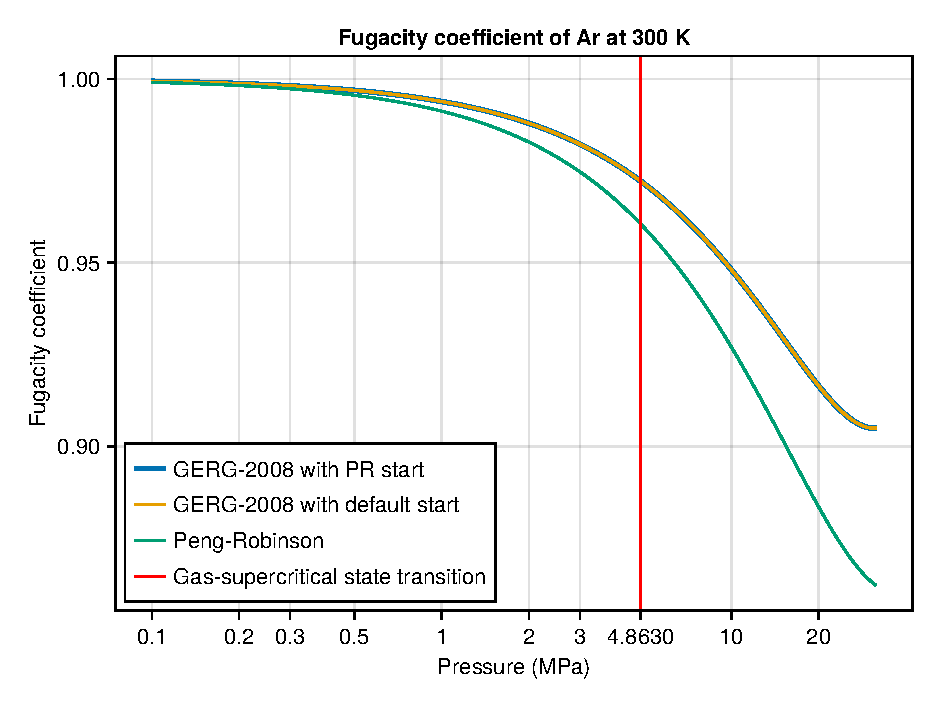
\includegraphics[width=\columnwidth]{figures/gcmc/fugacity_Ar.pdf}
		\subcaption{\ce{Ar} at \qty{300}K}
	\end{subfigure}\hfill%
	\begin{subfigure}{0.5\columnwidth}
		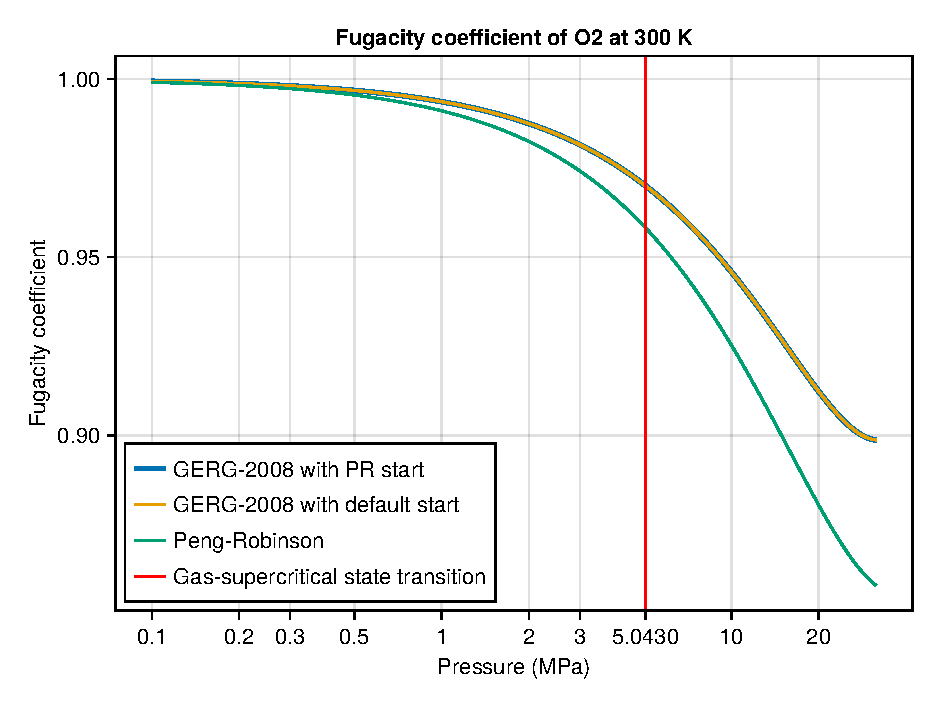
\includegraphics[width=\columnwidth]{figures/gcmc/fugacity_O2.pdf}
		\subcaption{\ce{O_2} at \qty{300}K}
	\end{subfigure}

	\caption{Fugacity coefficients of small gases computed with different \texttt{Clapeyron.jl} models}\label{fugacity}
\end{figure}

In terms of programming, the fugacity coefficient can directly be obtained from the \texttt{Clapeyron.jl} \autocite{Clapeyron} Julia package, which provides a convenient unified access to many useful thermodynamic tools. Due to the way it is implemented, Clapeyron.jl fails at finding the fugacity coefficient for \ce{CO_2} at high pressures: to solve this issue, we do an initial volume computation for the gas in the target conditions using the Peng-Robinson model, and we use the result as the starting point to compute the coefficient with the GERG-2008 model in Clapeyron. \Cref{fugacityCO2} illustrates the differences between these approaches: the latter allows to compute fugacities at any pressure except those very close to the critical point (\qty{304.13}K and \qty{7.3773}{MPa} for \ce{CO_2}), while the former simply fails at high pressures (above \qty1{MPa}). The other gases illustrated on \cref{fugacity} show that the Peng-Robinson fugacity is usually very close (less than \qty{5}\% difference) but systematically slightly lower than that obtained with GERG-2008, which would result in an equally slight shift of the isotherm. The difference between the two equations of state remains in the uncertainty margin of the GCMC simulation however, so it should not lead to a visible difference in the measured adsorption capacity.

\subsection{Computational aspects}

Compared to canonical MC, the efficient implementation of GCMC poses the additional challenge of changing the number of particles across the simulation. This requires almost no accommodation for the computations that operate in the real space, \textit{i.e.} framework pre-computed grids, and pairwise interactions (including the direct part of Ewald summation). For these, the only adaptation consists in making the neighbour lists resizable, which is already implemented in \texttt{CellListMap.jl}, and otherwise keeping the list of atoms in the system up to date, to correctly check each pair of atoms.

\subsubsection{Ewald summation}

Although the direct part of Ewald summation can be treated like the other short-range pair interactions, the reciprocal-space part of Ewald summation requires adapting the optimization described in \cref{energydifference} to account for the possible introduction or removal of a species. For such a move, both values of $S_{\boldsymbol k} = \sum_n q_ne^{-i\boldsymbol k\cdot\boldsymbol r_n}$ before and after the swap need to be computed, exactly like in \cref{eq:reciprocal_move}. Similar to that case, the value before the swap is already stored in memory, but the computation of the new value is slightly different: instead of computing the difference as $\sum_n q_n\paren{e^{-i\boldsymbol k\cdot\boldsymbol r'_n} - e^{-i\boldsymbol k\cdot\boldsymbol r_n}}$, the difference is now $\pm\sum_{n\text{ swapped}} q_n e^{-i\boldsymbol k\cdot\boldsymbol r_n}$. In the case of a deletion, each element of the latter is already stored in memory, whereas in the case of an insertion, this new computation is stored in a temporary place, like for any other trial move, ready to be stored permanently if the move is accepted.

The self-interaction term is no longer constant: each new molecule contributes a term equal to $-\sum_{m,n}\frac{q_n q_m}{8\pi\varepsilon_0}\text{erf}\paren{\pnorm{\boldsymbol r_n - \boldsymbol r_m}}/\pnorm{\boldsymbol r_n - \boldsymbol r_m}$ where $m$ and $n$ iterate over the atoms of the molecule with $m\neq n$. This term is computed once for each kind of molecules and stored, so that the contribution of the self-interaction term can be updated with a single addition or subtraction when a swap move occurs. Of course, any molecule whose number can vary in the system must be electrically neutral to ensure the the total system remains electrically neutral; this is also enforced in the code.

\subsubsection{Tail correction}

\label{tailcorrection}

Another difference is the tail correction, which is not constant anymore either. The tail correction, whose particular relevance for the particular context of porous materials modeling was exhibited by \textcite{TailCorrection}, is an approximation of the energy resulting from the pair interactions further than the cutoff: if the pair interaction is shifted in the force field, then this energy is null, but otherwise it needs to be taken into account.

To do so, a useful ansatz consists in assuming that the radial distribution function $g(r)$ is equal to 1 beyond the cutoff distance $r_c$, for all species. In turn, this allows analytically deriving the energy resulting from the average interaction of particles beyond the cutoff. For example, two particles interacting with a Lennard-Jones potential (see \cref{eq:LJ}) yield, for a unit cell volume $V$ and cutoff distance $r_c$, a tail correction of:
\[\text{tc}^\text{LJ} = \frac{8\pi}{3V}\varepsilon\sigma^3\times\paren{\frac13\paren{\frac{\sigma}{r_c}}^9 - \paren{\frac{\sigma}{r_c}}^3}\]
Similarly, two particles interacting with a Buckingham potential (see \cref{eq:Buckingham}) yield a tail correction of:
\[\text{tc}^\text{Buckingham} = \frac{2\pi}V \paren{A\exp(-Br_c)\times\frac{2 + Br_c(2 + Br_c)}{B^3} - \frac C{3r_c^3}}\]

All tail corrections $\text{tc}_{A,B}$ between one atom of kind $A$ and one of kind $B$ are precomputed for the given framework volume $V$ and cutoff $r_c$, and the total tail correction is the sum
\[\text{tc} = \sum_A\sum_B N_AN_B\text{tc}_{A,B}\]
where $N_A$ and $N_B$ are the number of atoms of kind $i$ and $j$. Knowing the number of each atom kind per molecule, it is thus possible to precompute the tail correction $\text{tc}(i,j)$ associated with each pair of molecule kinds $(i,j)$, as well as the tail correction $\text{tc}(i)$ due to the interaction of one molecule of kind $i$ and the framework. Those terms being precomputed, the total tail correction can be expressed as
\[\text{tc} = \text{tc}_\text{framework} + \sum_i \paren{n_i\text{tc}(i) + n_i^2\text{tc}(i,i)} + \sum_i\sum_{j\neq i} n_in_j\text{tc}(i,j)\]
where $\text{tc}_\text{framework}$ is the constant tail correction due to the interaction of the framework atoms with each other, and $n_i$, $n_j$ are the number of molecules of kinds $i$ and $j$.

Finally, the evolution of the tail correction when adding ($+$) or removing ($-$) one particle of kind $i$ is thus
\[\Delta_{\pm}\text{tc} = \pm\text{tc}(i) \pm\paren{2n_i\pm1}\text{tc}(i,i) \pm 2\sum_{j\neq i} n_j\text{tc}(i,j)\]

%\subsubsection{Excluded volume}
%
%As explained in \cref{blockingpockets}, atomic boolean grids are precomputed to fast-reject trial moves that would lead to a very high energy increase. The same method can be used to mark some specific parts of the framework as inaccessible, to prevent species from entering them when it would be kinetically unfeasible to do so.
%
%It stands to reason that a swap insertion move should also never create a new species in this excluded volume of the framework: there are two implementation possibilities to do so. The most direct one consists in continuing to choose an insertion position at random, and simply rejecting the trial move if the molecule happens to touch the excluded volume. This approach is correct but it leads to many rejections, so the simulation must run for long times to reach convergence. Instead, the alternative consists in only choosing insertion positions out of the excluded volume, by using a technique similar to that explained for the reinsertion moves.
%


\subsubsection{Resizable lists}

Overall, having a variable number of species requires extra bookkeeping, to make sure that all atoms are accounted for. To maximize performance in current computers, the data structures must have good cache locality: this means that, when memory needs to be read, it should be done in contiguous accesses as much as possible. For this purpose, the positions of the atoms, the $\kappa_{\boldsymbol k}$ factors, the precomputed $q_ne^{i\boldsymbol k\cdot \boldsymbol r_n}$ and $S_{\boldsymbol k}$ values, the self-interaction terms, etc., are all stored in tight arrays, with the appropriate indexing for each. When an atom or a molecule is removed, there are two choices, illustrated on \cref{fig:resizelist}: either leave a gap in the array, and keep track separately of which parts of the array actually refer to a valid data if need be, or move the contents of the array to fill the gap.

\begin{figure}
	\centering
	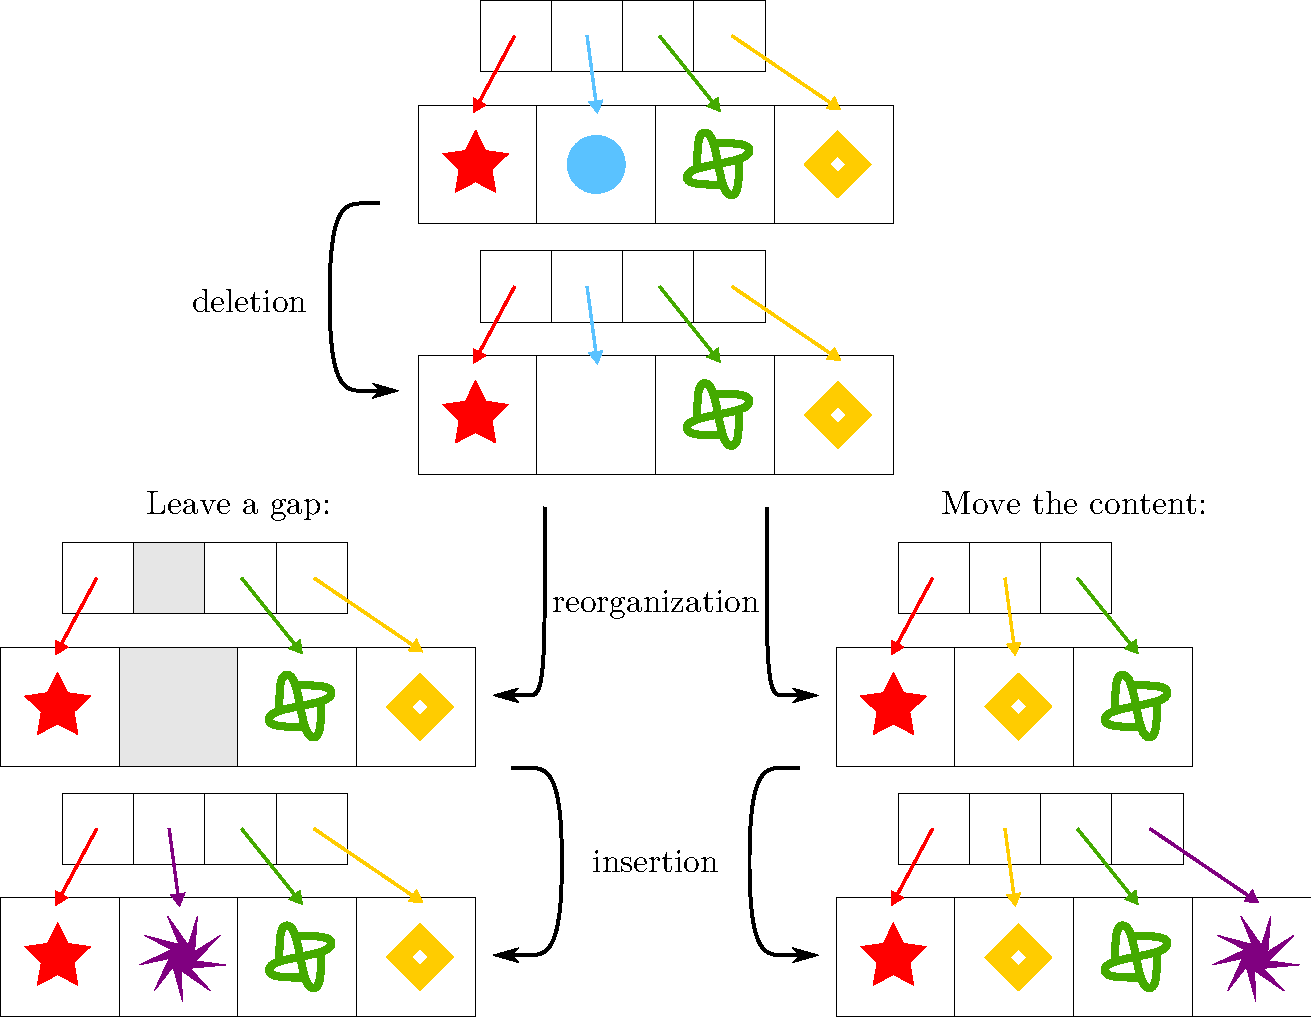
\includegraphics[width=\linewidth]{figures/gcmc/resizelist.pdf}
	\caption{Schematic representations of the list resizing algorithmic options}\label{fig:resizelist}
\end{figure}

Both algorithmic strategies have their merit, and warrant a trial to check which performs best. I did not take the time to implement both however, and instead chose the latter systematically, because it is slightly simpler to reason about. In practice, such an approach consists in replacing the content of the gap in the array by the data at the end of the array, before reducing the size of the array, and thus removing the temporarily duplicated data at the end. The indices relative to the content of the array also need to be updated. The complexity of each array update is thus proportional to the number of elements to remove, which is generally optimal. Insertions are operated at the end of the arrays, with an optimal complexity.

\section{GCMC on a grid}

Even with an efficient implementation, regular GCMC simulation remain resource-consuming, especially in the context of a large scale material screening. Improving this performance is thus valuable, especially if the precision cost can be controlled.

\subsection{Principle}

Similar to the methods exposed in \cref{precomputations}, a typical strategy for reducing the computational cost consists in precomputing as much as possible, to decrease the workload of the main loop of the algorithm. In the case of GCMC, the main computation occurring at each trial move is that of the interactions between species, both in direct and reciprocal spaces. Since the configuration space for the molecules in the unit cell of the framework is continuous, and thus infinite, it is impossible to precompute all the possible pair interactions.

However, that space can be discretized: to do so, the mobile species are forced to occupy one position each among a fixed set of possibilities. This principle is identical to the site hopping used in the case of cations (see \cref{sitehopping}) except that, as explained in \cref{adsorptionsites}, gas species are likely to occupy many more sites than cations. Thus, the conceptually simplest set of possible positions is a regular grid: each molecule must reside atop one grid point. For polyatomic species, like all gases of interest with the exception of rare gases, this definition is incomplete however, so there are three options, also illustrated on \cref{fig:3options}:
\begin{enumerate}
	\item[$\mathscr A$)] the grid can include additional dimensions to account for the orientation of the molecule. In that case there must be a fixed convention dictating which atom of the molecule is placed on the grid point. That atom, called the ``bead'', is typically that around which the rotation MC move operates.
	\item[$\mathscr B$)] each grid point can come with an associated fixed orientation of the molecule sitting on it. In that case, the lowest energy orientation with respect to the framework is probably the most reasonable choice, but it may grossly misrepresent the actual orientation of the molecules if those are mostly driven by the interaction with other molecules.
	\item[$\mathscr C$)] the molecule can be represented as a single point sitting on the grid, with no orientation. In that case, the interaction energy of the molecule with the framework can be taken as the average of the energies corresponding to the different orientations and, likewise, the molecule-molecule interactions can be computed by taking averages over the orientation of both molecules. These averages could be either arithmetic or Boltzmann averages, depending on the interpretation: a Boltzmann average implicitly assumes that the molecules are at equilibrium, which is not very well defined for a single molecule sitting on a grid point, while an arithmetic average implies has an orientation independent of the corresponding energy, which is not exact either.
\end{enumerate}

\begin{figure}
	\centering
	\hfill\begin{subfigure}{0.33\linewidth}
		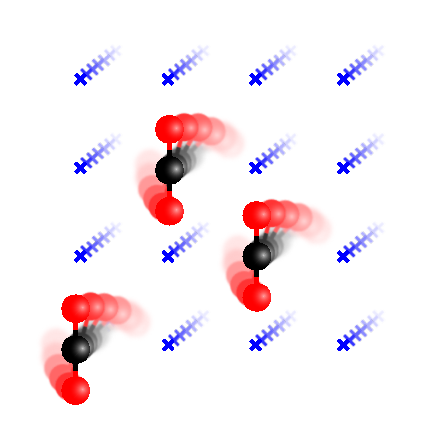
\includegraphics[width=1.05\linewidth]{figures/gcmc/gridMC_optionA.pdf}
		\subcaption{Option $\mathscr A$: explicit angles}
	\end{subfigure}\hfill%
	\begin{subfigure}{0.33\linewidth}
		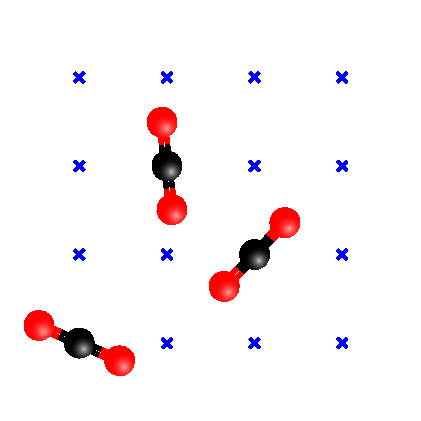
\includegraphics[width=1.05\linewidth]{figures/gcmc/gridMC_optionB.pdf}
		\subcaption{Option $\mathscr B$: single angle}
	\end{subfigure}\hfill%
	\begin{subfigure}{0.33\linewidth}
		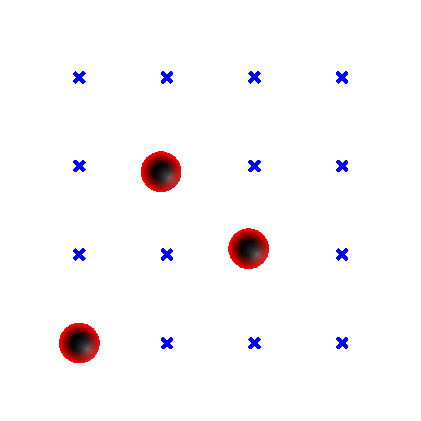
\includegraphics[width=1.05\linewidth]{figures/gcmc/gridMC_optionC.pdf}
		\subcaption{Option $\mathscr C$: averages}
	\end{subfigure}\hfill
	\caption{The three considered options to account for angles on a grid}\label{fig:3options}
\end{figure}

Our study is restricted to small gases of the air which are all linear and centrosymmetric: \ce{CO_2}, \ce{N_2}, \ce{O_2}, etc., so the bead is conventionally chosen as the center of the molecule. Choosing an orientation thus amounts to choosing a direction for a rod (the molecule) across all possible angles. To accurately cover this configuration space while limiting the number of studied angles, we use a Lebedev grid, which is a set of \Nleb points $(\theta_i,\varphi_i)$ on the surface of the sphere such that the integral of a function $f$ can be well approximated by the sum
\[I[f] = \int_0^\pi sin(\theta)\text d\theta \int_0^{2\pi}\text d\varphi f(\theta, \varphi)\ \approx\ 4\pi\sum_{i=1}^{\Nleb} w_if(\theta_i,\varphi_i)\]
with the appropriate weights $w_i$. The values of $w_i$, $\theta_i$ and $\varphi_i$ have been precomputed once and for all for different values of \Nleb. Because of orthogonality constraints on the Lebedev points, not all values of \Nleb are possible: the ones which are usable in my code are $\Nleb =$ 6, 14, 26, 38, 50, 74, 86, 110, 146, 170, 194, 230, 266, 302, 350, 434, 590, 770, 974, 1202, 1454, 1730, 2030, 2354, 2702, 3074, 3470, 3890, 4334, 4802, 5294 and 5810, allowing for any fine-tuning of the precision level. Only half of these points are actually used since the both the target gases and the Lebedev grids are centrosymmetric. A few representations of the Lebedev grid are given on \cref{fig:lebedev}

\begin{figure}
	\centering
	\begin{minipage}{0.55\linewidth}
		\begin{subfigure}{0.5\linewidth}
			\centering
			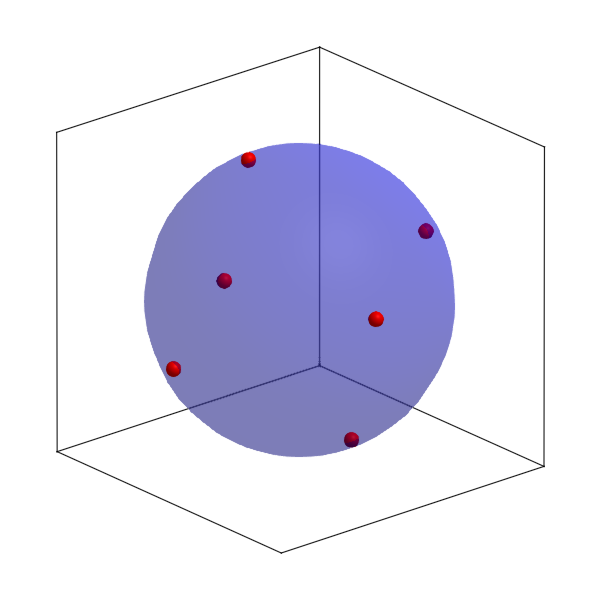
\includegraphics[width=\linewidth]{figures/gcmc/lebedev_6}
			\caption{6 points}
		\end{subfigure}%
		\begin{subfigure}{0.5\linewidth}
			\centering
			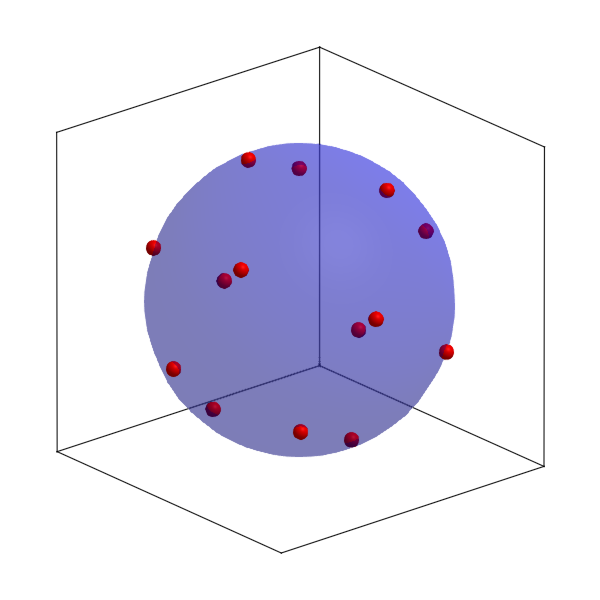
\includegraphics[width=\linewidth]{figures/gcmc/lebedev_14}
			\caption{14 points}
		\end{subfigure}

		\begin{subfigure}{0.5\linewidth}
			\centering
			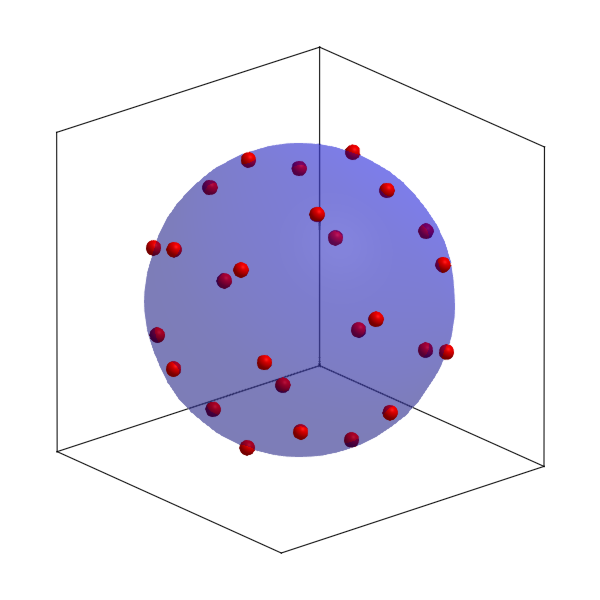
\includegraphics[width=\linewidth]{figures/gcmc/lebedev_26}
			\caption{26 points}
		\end{subfigure}%
		\begin{subfigure}{0.5\linewidth}
			\centering
			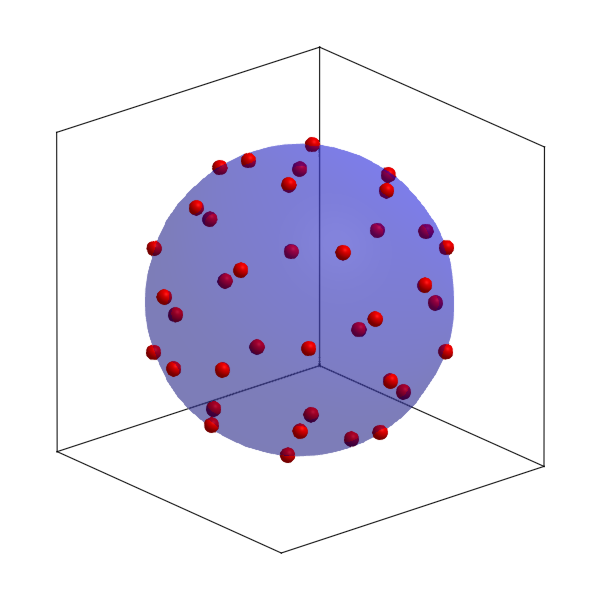
\includegraphics[width=\linewidth]{figures/gcmc/lebedev_38}
			\caption{38 points}
		\end{subfigure}
	\end{minipage}%
	\begin{minipage}{0.45\linewidth}
		\begin{subfigure}{\linewidth}
			\centering
			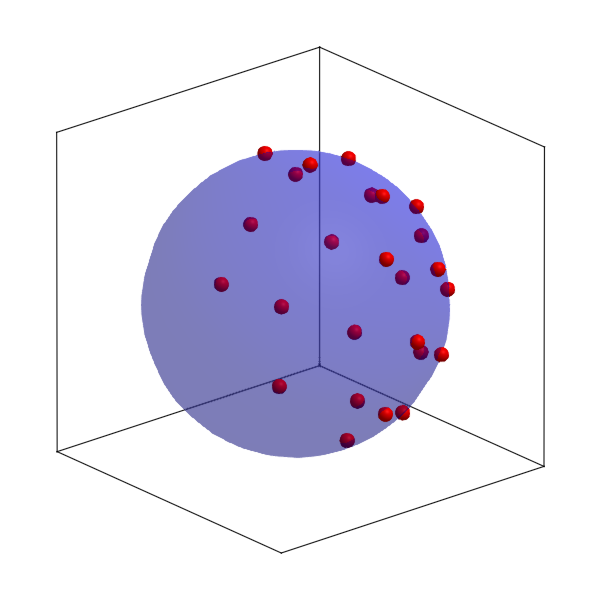
\includegraphics[width=\linewidth]{figures/gcmc/lebedev_25_symm}
			\caption{25 points half grid}\label{fig:haldgridlebedev}
		\end{subfigure}
	\end{minipage}

	\caption{Lebedev grid points. \cref{fig:haldgridlebedev} is a half grid, used for centrosymmetric species.}\label{fig:lebedev}
\end{figure}

The number of possible configurations of a molecule is $\alpha\times a\times b\times c$ where $(a,b,c)$ is the size of the spatial grid and $\alpha$ is either \Nleb in option $\mathscr A$, or 1 for options $\mathscr B$ and $\mathscr C$. Since we use a Van der Waals cutoff of \qty{12}\angstrom, the framework with the smallest grid will necessarily have its perpendicular lengths greater or equal to $2\times\qty{12}\angstrom = \qty{24}\angstrom$. Thus, with a distance of \qty{0.2}{\angstrom} between two grid points, $a$, $b$ and $c$ are greater or equal to $120$ so the size of the configuration space is at least $\alpha\times120^3$.

The goal of the grid MC approach is to reduce the amount of computations done at each step to accelerate the GCMC simulations, by precomputing the pair interactions between grid points. The number of pair interactions to precompute is thus, in theory, at least $\paren{\alpha\times120^3}^2/2 = \alpha^2\times120^6/2$. It can actually be reduced further with translation symmetry considerations: the interaction between grid points $(x_1,y_1,z_1,\theta_1)$ and $(x_2,y_2,z_2,\theta_2)$ is identical to that between grid points $(x_1+\Delta,y_1+\Delta,z_1+\Delta,\theta_1)$ and $(x_2+\Delta,y_2+\Delta,z_2+\Delta,\theta_2)$ for any $\Delta$. It is thus sufficient to precompute the interaction between $(0,0,0,\theta)$ and all other grid points, so the minimum number of precomputations is actually $\alpha^2\times 120^3 \approx \alpha^2\times 2\cdot10^6$. Each precomputation yields an energy, represented by a floating-point number, which takes \qty8B of space, and the typical RAM of a computer is on the order of \qty{10}{GB}, so the maximum value of $\alpha$ is approximately $\sqrt{10^{10}/\paren{8\times 2\cdot10^6}} = 25$ for the smallest possible spatial grid.

In conclusion, using explicit angles (option $\mathscr A$) is theoretically doable only for small enough materials and by using the smallest numbers of angles, otherwise the precomputation results cannot be stored in memory. Moreover, the numerical cost of the precomputation itself can be expected to be considerable, since it requires $\alpha^2\times 2\cdot10^6$ pair interaction computations. This is similar to the cost of simulating a system of $N = \alpha^2$ particles in interaction across one million MC steps (which is close to a typical GCMC simulation length), since each MC trial move requires computing $2N$ pair interactions ($N$ for the particle before the move, $N$ for the particle after). Therefore, option $\mathscr A$ is unlikely to be applicable in many cases.

\subsection{Validation}

\begin{figure}
	\centering
	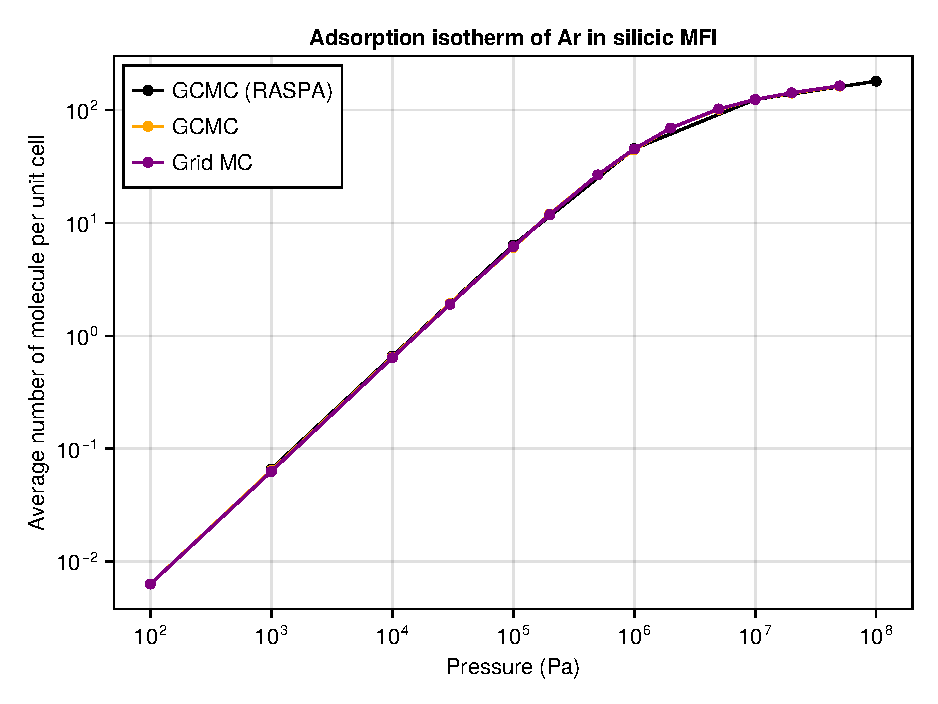
\includegraphics[width=0.8\columnwidth]{figures/gcmc/gridmc_Ar_MFI.pdf}
	\caption{Adsorption isotherm of Ar on silicic MFI obtained with different simulation strategies. The black line is the RASPA implementation of GCMC while the orange line is my implementation.}\label{fig:gridMC-ArMFI}
\end{figure}

To check the validity of this simulation strategy, we start by comparing the loading of Ar in a zeolite obtained by regular GCMC and through this grid MC approach. The result for zeolite MFI is presented on \cref{fig:gridMC-ArMFI}, using a grid step size of \qty{0.2}{\angstrom}. The perfect superposition of the three isotherms indicate that the grid MC simulation method is apt to reproduce the adsorption property of noble gas in zeolites with great accuracy, even at high pressure.

With more complex molecules, angles have to be taken into account, using either option $\mathscr B$ or $\mathscr C$. Their comparison is illustrated with the adsorption of \ce{CO_2} in FAU in \cref{fig:gridMC-pair}, shows that averaging orientations ($\mathscr C$) provide more qualitative results compared to selecting one single orientation per grid point ($\mathscr B$). Yet, none manage to qualitatively reproduce the adsorption behavior at medium/high pressures.

\begin{figure}
	\centering
	\begin{subfigure}{0.93\columnwidth}
		\centering
		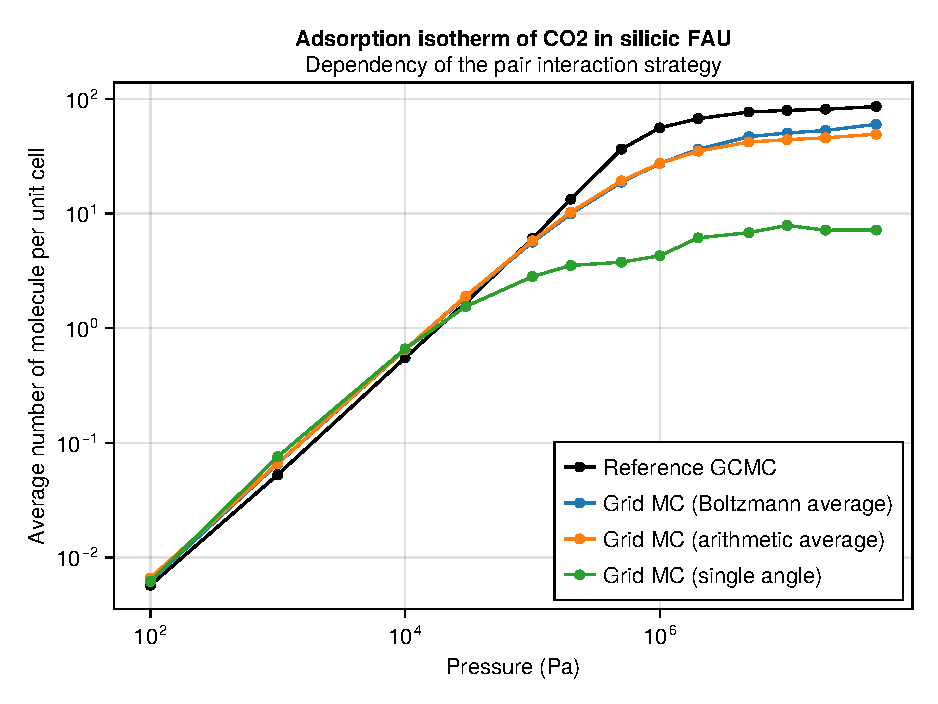
\includegraphics[width=0.86\columnwidth]{figures/gcmc/gridmc_CO2_FAU_comparison_pair.pdf}
		\subcaption{Influence of the molecule-molecule interaction strategy. ``single angle'' refers to option $\mathscr B$, while for option $\mathscr C$, the fixed framework-molecule interaction strategy is the Boltzmann average.}\label{fig:gridMC-pair}
	\end{subfigure}

\vspace{2em}

	\begin{subfigure}{0.93\columnwidth}
		\centering
		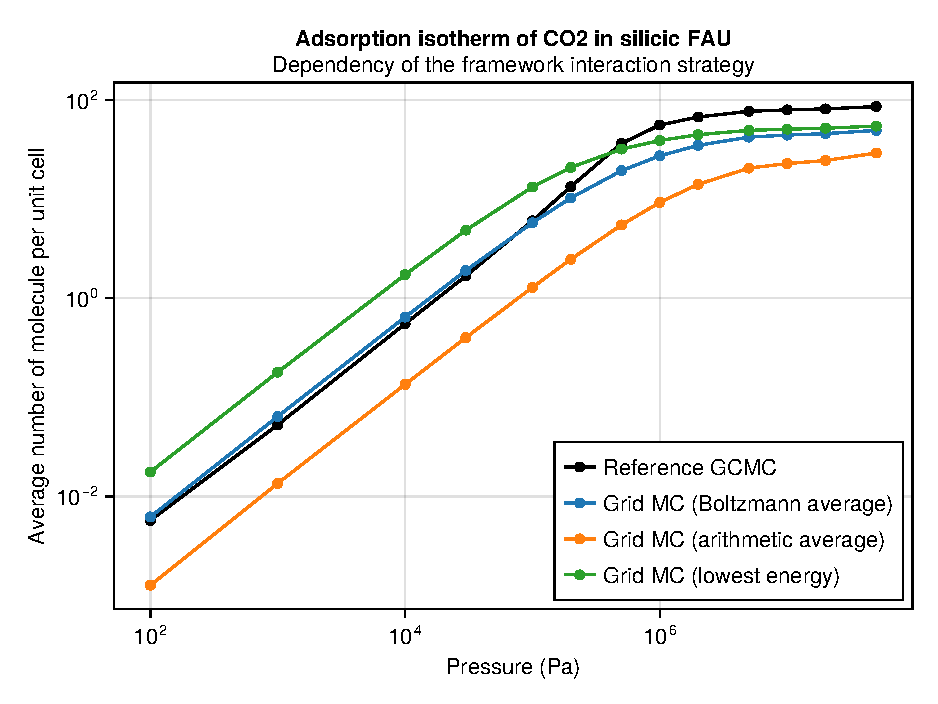
\includegraphics[width=0.86\columnwidth]{figures/gcmc/gridmc_CO2_FAU_comparison_framework.pdf}
		\subcaption{Influence of the framework-molecule interaction strategy with option $\mathscr C$. The fixed molecule-molecule interaction strategy is the arithmetic average. ``lowest energy'' refers to taking the minimum instead of taking an average.}\label{fig:gridMC-framework}
	\end{subfigure}
	
	\caption{Adsorption isotherm of \ce{CO_2} on silicic FAU obtained with different grid MC strategies.}\label{fig:gridMC-comparison}
\end{figure}


As evoked previously, the nature of the angular averaging of energies, either arithmetic or Boltzmannian, stems from a hypothesis on the distribution of microstates, neither of which is actually valid. The influence of this choice on the simulated loading of \ce{CO_2} in FAU is presented in \cref{fig:gridMC-comparison}.

In \cref{fig:gridMC-pair}, it appears that the choice of averaging for the molecule-molecule interaction has little influence on the result until the high pressures. Unsurprisingly, the Boltzmann average, which favors attractive interaction, increases the loading compared the arithmetic average, but the general trend is very similar and neither appear to be particularly more right than the other.

On the other hand, \cref{fig:gridMC-framework} illustrates the drastic difference in the choice of averaging for the framework-molecule interaction. Only the Boltzmann average yields an isotherm closely following that of the reference GCMC simulation at low pressures: the arithmetic averaging of angles yields a large underestimation of the loading, while taking only the lowest energy across angles yields a large overestimation.

From these observations, it appears that the molecules of \ce{CO_2} preferentially orient themselves according to the interactions with the framework at low pressure, which should be obvious since low pressures correspond to a regime where molecule-molecule interactions are negligible. More importantly, irrespective of the pressure regime, the entropic contribution is paramount: the molecules do not simply orient themselves according to the lowest energy configuration, but freely rotate in accordance with Boltzmann distribution.

\begin{figure}
	\centering
	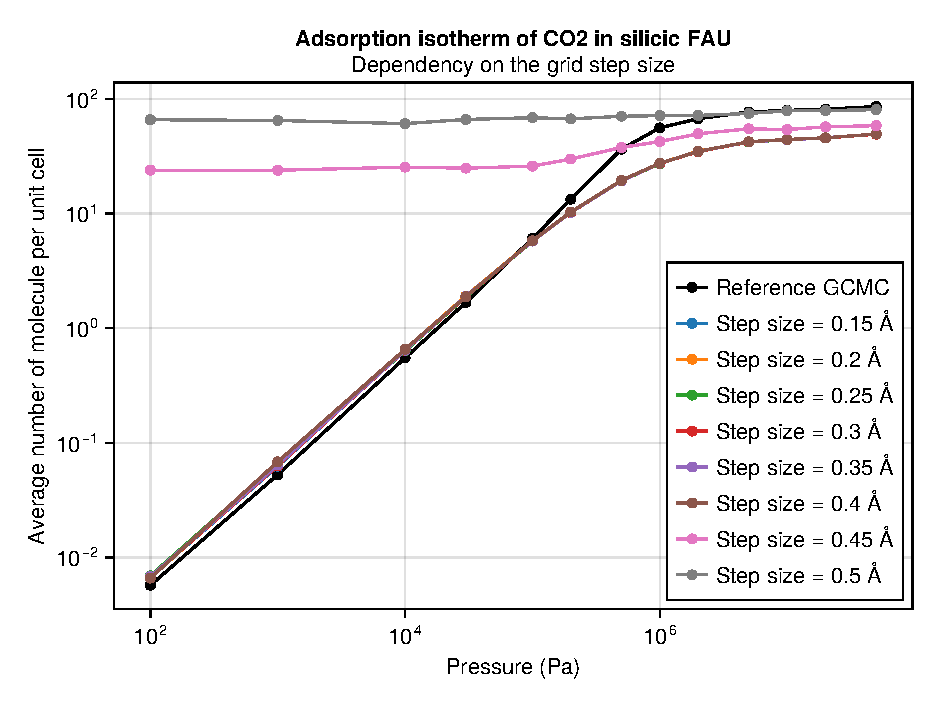
\includegraphics[width=0.8\columnwidth]{figures/gcmc/gridmc_CO2_FAU_comparison_size.pdf}
	\caption{Adsorption isotherm of \ce{CO_2} on silicic FAU obtained with different grid MC step sizes}\label{fig:gridMC-sizes}
\end{figure}

Regarding the numerical method itself, the main limit is the behaviour at intermediate and high pressure, which significantly parts from expectation. While this necessarily stems from the use of a grid, it does not depend on the grid step size: \cref{fig:gridMC-sizes} shows the evolution of the isotherm using option $\mathscr C$ with Boltzmann averaging for framework-molecule interactions and arithmetic averaging for molecule-molecule interactions. The isotherm remains constant as long as the grid step size is small enough, which points to the fact the issue lies in the nature of the simulation method itself.

\subsection{Computational aspects}

The main interest of the grid MC approach is that all pair interaction energies can be precomputed, which makes each trial move much less computationally costly, and thus the overall simulation much faster. Indeed, the variation of energy due to a single MC trial move can be expressed as
\[\Delta E^\text{grid MC} = \left\{\begin{split}
	\delta(N+1, \boldsymbol r)\ &\text{if insertion of a new molecule at }\boldsymbol r\\
	-\delta(i, \boldsymbol r)\ &\text{if deletion of the molecule }i\text{ at }\boldsymbol r\\
	\delta(i, \boldsymbol r') - \delta(i, \boldsymbol r)\ &\text{if move of the molecule }i\text{ from }\boldsymbol r\text{ to }\boldsymbol r'
\end{split}\right.\]
where $N$ is the number of molecules in the system and
\[\delta(i, \boldsymbol r) = \text{framework}(\boldsymbol r) + \sum_{j\neq i} \text{interaction}(\boldsymbol r, \boldsymbol r_j) + \text{tc}_\text{framework} + (2N+1)\text{tc}_\text{interaction}\]

The different terms above are all precomputed for the different values of the grid point $\boldsymbol r$:
\begin{itemize}
	\item $\text{framework}(\boldsymbol r)$ refers to the framework-molecule interaction, which is computed once and for all according to either of the three options $\mathscr A$, $\mathscr B$ and $\mathscr C$ discussed before.
	\item $\text{interaction}(\boldsymbol r, \boldsymbol r')$ is the interaction between two molecules, one at $\boldsymbol r$ and the other at $\boldsymbol r'$.
	\item $\text{tc}_\text{framework}$ is the tail correction for the atoms of the framework and the atoms of the molecule, and $\text{tc}_\text{interaction}$ is the tail correction for the atoms of two molecules interacting.
\end{itemize}

The tail correction terms are stored as simple numbers, $\text{framework}(\boldsymbol r)$ is stored as a tridimensional array of energies, $\boldsymbol r$ being mapped to a triplet of integers indexing the grid points. The term that takes the most time to precompute, $\text{interaction}(\boldsymbol r, \boldsymbol r')$, is stored in a custom data structure made of a tridimensional index array, along the energy data, in a flat list. Due to translation symmetry, the query of the interaction between $\boldsymbol r$ and $\boldsymbol r'$ becomes that between the origin and $\boldsymbol r - \boldsymbol r'$. The corresponding triplet of integers maps to an index in the tridimensional array, and that index is the one used to retrieve the energy from the energy list. The index can also be 0, to indicate that the interaction energy is zero (i.e. beyond the cutoff): this way, the energy list only stores relevant values.

The precomputation itself is also optimized, to avoid making it the dominant computational cost of running grid MC simulations. To do so, the framework interactions computation benefits from all the precomputations explained in \cref{precomputations}, in particular the tabulated atomic grids. For the molecule-molecule interaction averaged over the angles, the energy is interpolated from a linear grid: the interaction energy is computed by putting the bead of the first molecule at the origin and the other at a distance $d$, where $d$ increments from 0 to the cutoff distance by steps of one fifth of the average MC grid step. The interpolation is done with cubic splines through the \texttt{BasicInterpolators.jl} Julia package.


\end{document}
